\documentclass{article}

\usepackage[utf8]{inputenc}
\usepackage[english]{babel}
\usepackage{hyperref}
\usepackage{amsmath}
\usepackage{float}
\usepackage{cite}
\usepackage{url}
\usepackage{listings}
\usepackage{graphicx}
%\usepackage{parskip}
\usepackage{color}
\usepackage{tabularx}
\usepackage{booktabs}
\usepackage{titlesec}
\usepackage{geometry}
\usepackage[T1]{fontenc}

\hypersetup{
    hidelinks,
    colorlinks,
    urlcolor=blue,
    citecolor=[rgb]{0,.6,.25}
}

\newgeometry{vmargin={20mm}, hmargin={35mm,35mm}}

% https://tex.stackexchange.com/questions/60209/how-to-add-an-extra-level-of-sections-with-headings-below-subsubsection
\setcounter{secnumdepth}{4}

\titleformat{\paragraph}
{\normalfont\normalsize\bfseries}{\theparagraph}{1em}{}
\titlespacing*{\paragraph}
{0pt}{3.25ex plus 1ex minus .2ex}{1.5ex plus .2ex}

\definecolor{codegreen}{rgb}{0,0.6,0}
\definecolor{codegray}{rgb}{0.5,0.5,0.5}
\definecolor{codepurple}{rgb}{0.58,0,0.82}
\definecolor{backcolour}{rgb}{0.95,0.95,0.92}
\definecolor{lightgray}{rgb}{.9,.9,.9}
\definecolor{darkgray}{rgb}{.4,.4,.4}
\definecolor{purple}{rgb}{0.65, 0.12, 0.82}

\graphicspath{ {../assets/} }

\bibliographystyle{unsrt}

\lstdefinelanguage{JavaScript}{
    keywords={break, case, catch, continue, debugger, default, delete, do, else, false, finally, for, function, if, in, instanceof, new, null, return, switch, this, throw, true, try, typeof, var, void, while, with},
    morecomment=[l]{//},
    morecomment=[s]{/*}{*/},
    morestring=[b]',
    morestring=[b]",
    ndkeywords={class, export, boolean, throw, implements, import, this},
    keywordstyle=\color{blue}\bfseries,
    ndkeywordstyle=\color{darkgray}\bfseries,
    identifierstyle=\color{black},
    commentstyle=\color{purple}\ttfamily,
    stringstyle=\color{red}\ttfamily,
    sensitive=true
}
\lstdefinestyle{default}{
    backgroundcolor=\color{backcolour},
    commentstyle=\color{codegreen},
    keywordstyle=\color{magenta},
    numberstyle=\tiny\color{codegray},
    stringstyle=\color{codepurple},
    basicstyle=\ttfamily\footnotesize,
    breakatwhitespace=false,
    breaklines=true,
    captionpos=b,
    keepspaces=true,
    numbers=left,
    numbersep=5pt,
    showspaces=false,
    showstringspaces=false,
    showtabs=false,
    tabsize=2
}
\lstset{
    language=JavaScript,
    backgroundcolor=\color{lightgray},
    extendedchars=true,
    basicstyle=\footnotesize\ttfamily,
    showstringspaces=false,
    showspaces=false,
    tabsize=2,
    breaklines=true,
    showtabs=false,
    captionpos=b
}
\newcommand*{\fullref}[1]{\hyperref[{#1}]{\ref*{#1}~\nameref*{#1}}}
\makeatletter
\renewcommand\listoffigures{%
        \@starttoc{lof}%
}
\renewcommand\listoftables{%
        \@starttoc{lot}%
}
\renewcommand\lstlistoflistings{%
        \@starttoc{lol}%
}
\makeatother


\title{
    Decibel Threshold Event Displayer\\
    ~\\
    \large
    \textbf{Analyze Audio Files and detect Noise Pollution}
}
\author{
    Dominic Gernert (gernd1) \\
    Darius Degel (deged2) \\
    Lukas von Allmen (vonal3)
}
\date{\today}

\begin{document}
    \maketitle

\begin{table}[H]
    \centering
    \begin{tabularx}{\textwidth}{l X}
        \toprule
        School           & \textbf{Bern University of Applied Sciences} \\
        \midrule
        Module           & \textbf{BTI3031 - Project 1 (24/25)} \\
        \midrule
        Tutor            & \textbf{Dr. Simon Kramer} \\
        \bottomrule
    \end{tabularx}
    \label{tab:title-page}
\end{table}

\pagebreak
    \begin{abstract}\label{sec:abstract}

Noise pollution affects one in seven people in Switzerland, 
primarily caused by road traffic, railways, and air traffic, along with secondary sources such as construction sites and nightclubs. 
To address this issue, affected individuals must provide evidence, typically through audio recordings.
This project aims to create a free, open-source, and platform-independent application, which helps individuals in documenting noise pollution. \\
\\
The application processes *.WAV files, filters the data by a given threshold and
generates a PDF with an according plot which can be used as evidence.
For a meaningful interpretation of a *.WAV file, the user must provide a minimal and maximal dB(A) provided by an external tool,
such as smartphone apps like DecibelX. \\

\begin{table}[H]
    \centering
    \begin{tabularx}{\textwidth}{l X}
        \toprule
        License           & \textbf{\href{https://www.gnu.org/licenses/gpl-3.0.en.html}{GPL-3.0 licence (FLOSS)}} \\
        \midrule
        Application       & \textbf{\href{https://decibel-threshold-event-displayer.github.io/\#/}{dB threshold event displayer}} \\
        \midrule
        About Page        & \textbf{\href{https://decibel-threshold-event-displayer.github.io/\#/about}{About Decibel Threshold Event Displayer}} \\
        \midrule
        Repository        & \textbf{\href{https://github.com/decibel-threshold-event-displayer/decibel-threshold-event-displayer.github.io}{GitHub}} \\
        \bottomrule
    \end{tabularx}
    \label{tab:abstract-infos}
\end{table}

\-
%~\\

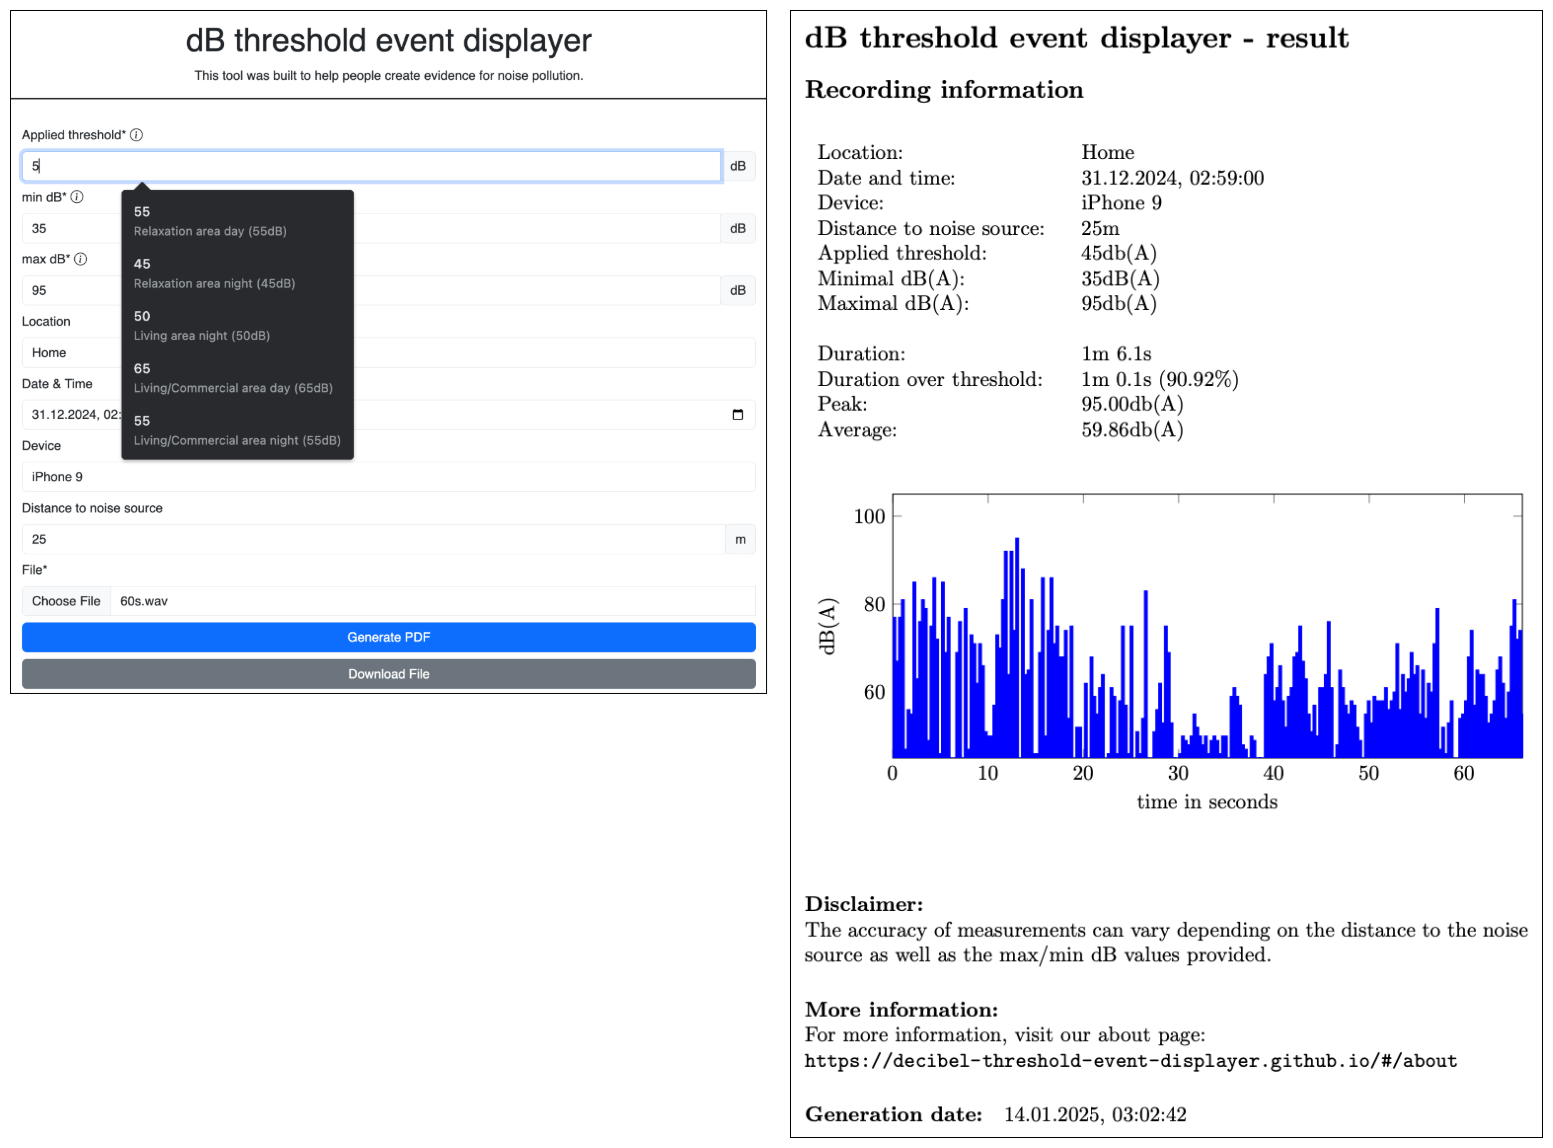
\includegraphics[width=0.8\textwidth]{../assets/abstract_preview.png}

%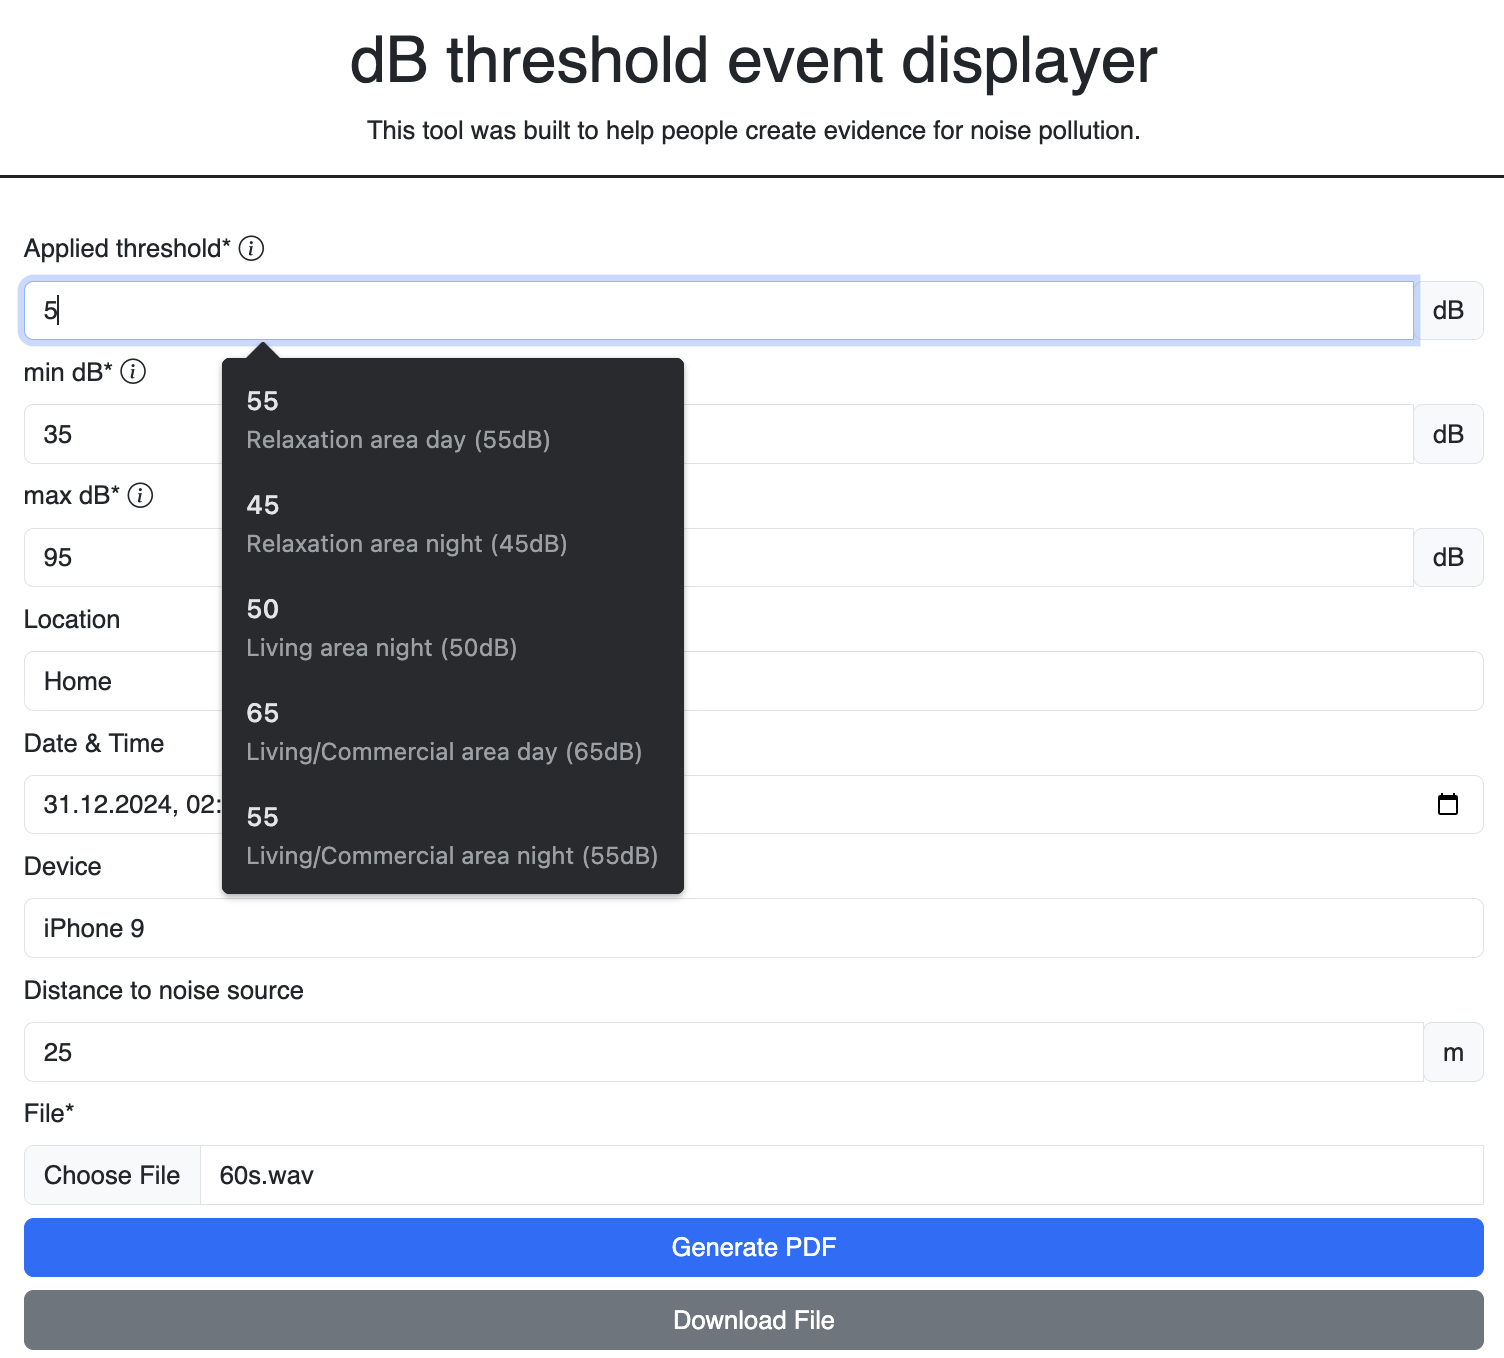
\includegraphics[width=0.475\textwidth]{../assets/abstract_application_screenshot.png}
%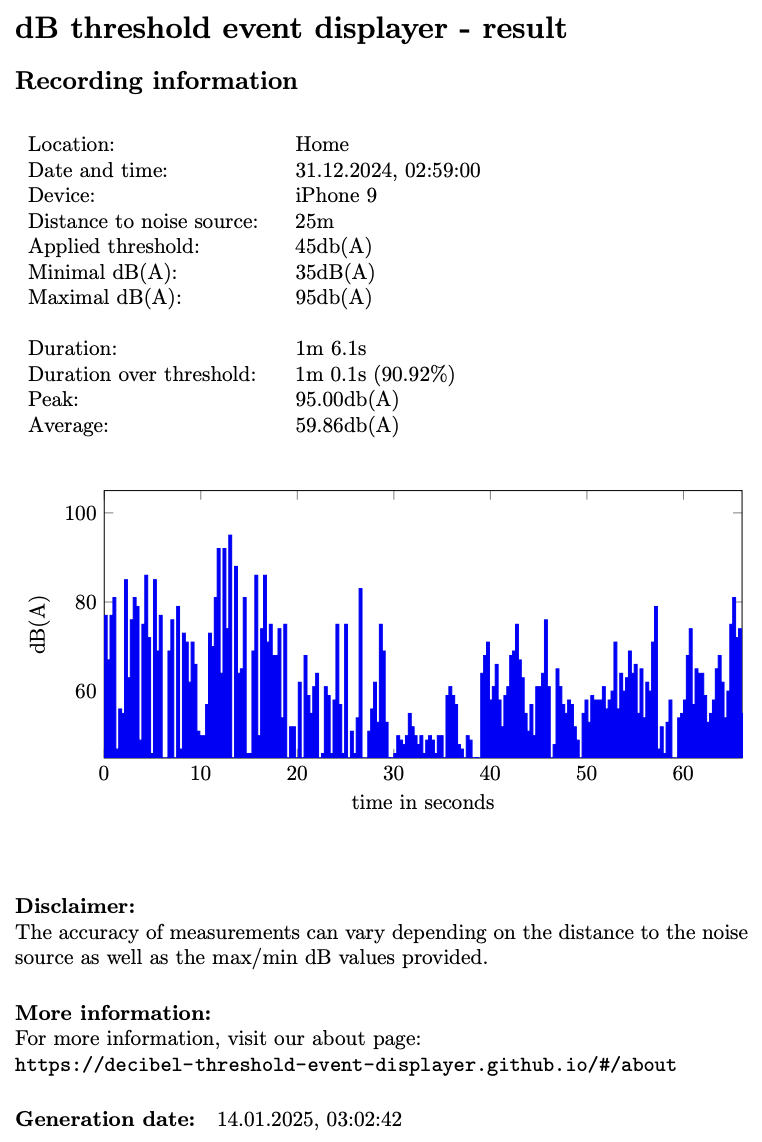
\includegraphics[width=0.475\textwidth]{../assets/abstract_report_screenshot.png}

\pagebreak
\end{abstract}
    \begingroup
    \hypersetup{hidelinks}
    \renewcommand\contentsname{Table of Contents}
    \tableofcontents
    \endgroup
    \section{List of Tables}

\begingroup
\hypersetup{hidelinks}
\listoftables
\endgroup
    \section{List of Figures}
\begingroup
\hypersetup{hidelinks}
\listoffigures
\endgroup
    \section{List of listings (code snipptes)}
Lorem ipsum

    \part{Product Documentation}
    \section{Introduction}\label{sec:introduction}

\subsection{Initial Situation}\label{subsec:initial-situation}
According to the~\href{https://www.bafu.admin.ch//}{Federal Office for the Environment} (DE:\ BAFU) one in seven people in Switzerland is affected by noise pollution~\cite{foen_noise_pollution}.
The pollution comes primarily from road traffic, followed by railways and then air traffic.
In addition to these noise sources, construction sites, nightclubs and public facilities also produce noise.
Because of this, Switzerland has set up upper noise limits that must be respected.
However, it is of course the case that these limits are not always adhered to.
Affected people must then either accept this or take action against it.
For the latter, they must gather evidence to prove their noise disturbance to the police and the courts.
This evidence then comes from an audio recording which the affected person made them self.

\subsection{Project Goal}\label{subsec:project-goal}
To help the people affected by noise pollution, we want to create an application which processes a given sound file (.wav)
and analyzes it.
It should detect when a specified threshold has been exceeded and then summarizes the result in a PDF document.
The document should then contain all necessary information for filing a complaint.
As our application will have a wide range of end users, two of our main design goals are to make it as user-friendly as possible
and to make it platform independent, so it can be used with any PC operating system and ideally mobile device.

\subsection{Problems with Audio Files}\label{subsec:problems-with-audio-files}
A wave file (.wav) contains samples of the recorded audio, where each sample represents the amplitude at a given moment.
Those amplitude values are relative to each other and not absolute.
It is therefore impossible to determine the actual dB(A) (loudness relative to the human ear) someone would perceive without any further information~\cite{adobe_community_how_to_know_the_real_world_db_level_of_a_file,stackoverflow_how_can_i_calculate_audio_db_level,stackexchange_exteracting_sound_pressure_from_wav_file}.
Because of this, we require the user to also give information about the minimal and maximal dB(A) measured in the given audio file.
To do this, we recommend using a smartphone app like \href{https://apps.apple.com/ch/app/dezibel-x-dba-l\%C3\%A4rm-messger\%C3\%A4t/id448155923}{DecibelX for IOS},
which allows the user to record the audio and also conveniently inspect the minimal and maximal dB measured in that recording.
With those two values, we can then map the relative values from the wave file to its db(A) values.
    \section{Specification}
The following chapter describes the system specification. The specification is derived from the requirements in the project description
as well as the discussions with the stakeholder. Assumptions and constraints are described in the following sections and were validated by
the defined product owner and the stakeholders if necessary.

\subsection{System Delimitation}
The system delimination is split into the static system environment (\ref{subsubsec:system_environment})
and the dynamic process environment (\ref{subsubsec:process_environment}).

\subsubsection{System Environment}
\label{subsubsec:system_environment}
System:
\begin{itemize}
    \item Frontend (User interaction)
    \item LaTeX and pgfplots
\end{itemize}
System context:
\begin{itemize}
    \item Stakeholder (tutor)
    \item User
    \item Lärmliga
    \item (Accurate conversion to absolute decibel)
\end{itemize}
Out of scope:
\begin{itemize}
    \item Integration in legal complaints
    \item (Accurate conversion to absolute decibel)
\end{itemize}

\subsubsection{Process Environment}
\label{subsubsec:process_environment}
\begin{itemize}
    \item Selecting a file
    \item WAV file analysis (validation, parsing, conversion to absolute db values, threshold filtering)
    \item Plotting (LaTeX / pgfplots) and PDF generation
\end{itemize}

\subsection{Requirements}
In the following section the requirements are detailed. Also the project boundaries and pre-conditions are described.

\subsubsection{Functional requirements}
The project team identified the following functional requirements:
\begin{table}[H]
    \centering
    \begin{tabularx}{\textwidth}{|c|X|c|c|c|}
        \hline
        \textbf{ID} & \textbf{Requirement} & \textbf{Priority} \\
        \hline
        R1 & Allow users to upload a .wav audio file. & MUST \\
        \hline
        R2 & Validate the uploaded file to ensure it is in .wav format, providing an error message if it is not. & MUST \\
        \hline
        R3 & Analyze the uploaded .wav file and calculate the noise level in decibels (dB). & MUST \\
        \hline
        R4 & Allow users to download the plotted noise data as an image or PDF. & MUST \\
        \hline
        R5 & Allow users to input metadata for the audio file, such as location, date, and time. & MUST \\
        \hline
        R6 & Plot the noise level data over time, with the x-axis representing time and the y-axis representing noise level (in dB). & MUST \\
        \hline
        R7 & Generate a PDF report including the plotted noise data and user input metadata. & MUST \\
        \hline
        R8 & Provide clear feedback and error messages. & SHOULD \\
        \hline
        R9 & Intuitive and responsive UI for selecting files, configuring options, and viewing results. & SHOULD \\
        \hline
        R10 & Allow the user to configure custom thresholds for noise levels. & COULD \\
        \hline
        R11 & Allow the user to change the language of the application. & COULD \\
        \hline
    \end{tabularx}
    \caption{Functional Requirements}
    \label{table:functional_requirements}
\end{table}

\subsubsection{Pre-Conditions and Boundaries}
Research done by the project team has revelead that reading absolute decibel values from WAV-files is more difficult than anticipated.
The reason for this is that normal consumer microphones are not calibrated for scientifically accurate measurements\cite{stackoverflow_spl}. Furthermore, it is trivial for a user
to increase the volume of a WAV-file using free, easy-to-use software like Audacity\cite{audacity}\cite{audacity_amplify}. Therefore, the project team has decided 
on a tentative working hypothesis together with the Stakeholder. \\ \\
Pre-Conditions:
\begin{itemize}
    \item The user must use a properly calibrated microphone or use a phone app which has built-in calibrations like Decibel X\cite{decibelx_ios}\cite{decibelx_android}.
    \item The user must have a way to export their audio recording as a WAV-file.
    \item The user must have access to a web browser capable of running WebAssembly.
    \item The user must not edit the exported WAV-file in any way except to decrease the length of the recording.
\end{itemize}
Boundaries:
\begin{itemize}
    \item The application supports only the analysis of pre-calibrated, un-edited WAV-files.
    \item The application supports only single-channel WAV-files.
    \item The user is presumed to be using properly calibrated equipment. There is no validation done in the application to ensure proper calibration.
    \item The user is presumed to be honest and to not have edited the WAV-file. There is no validation done in the application to ensure the file has not been edited.
\end{itemize}

\subsection{Usability}
Lorem ipsum

\subsubsection{Personas}
Lorem ipsum

\subsubsection{Storyboard}
Lorem ipsum

\subsubsection{UX-Prototyping}
Lorem ipsum
    \section{Evaluation}\label{sec:evaluation}

\subsection{Technology stack}\label{subsec:technology_stack}
Since the project description does not mention specific technologies to be used except for the LaTeX package pgfplots,
the project team decided to evaluate different technologies for the project by creating working prototypes.
The following chapters describe the evaluation criteria and the results of the evaluation.

\subsubsection{Criteria}
The following criteria are used to decide which technologies should be used for the project:
\begin{itemize}
    \item Know-how (10\%)
    \item Complexity (20\%)
    \item Usability (30\%)
    \item Distribution (40\%)
\end{itemize}

\subsubsection{Calculation}
The formula for calculating the weighted value of each criterion is:
\[
    v_w = \text{weight} \cdot \frac{\text{evaluation}}{5}
\]
Where \(evaluation\) is the scoring between 1--5.
The total score for a given technology is the sum
of weighted values.

\subsubsection{Technologies}
The following technologies were evaluated:
\begin{itemize}
    \item Kotlin with pdflatex as a dependency
    \item Kotlin bundled with pdflatex
    \item Website with SwiftLaTeX
\end{itemize}

\subsubsection{Reference LaTeX pgfplots template}\label{subsec:reference_latex_pgfplots_template}
For building the prototypes we will use the following reference LaTeX template which includes a pgfplots object:~\cite{pgfplots_gallery_sourceforge}

\begin{lstlisting}[caption={Reference LaTeX template with a pgfplots object},label={lst:reference_latex_pgfplots_template},language={[LaTeX]{TeX}}]
\documentclass{article}

\usepackage{siunitx}
\usepackage{tikz} % To generate the plot from csv
\usepackage{pgfplots}

\pgfplotsset{compat=newest} % Allows to place the legend below plot
\usepgfplotslibrary{units} % Allows to enter the units nicely

\sisetup{
  round-mode          = places,
  round-precision     = 2,
}

\begin{document}

\begin{figure}[h!]
  \begin{center}
    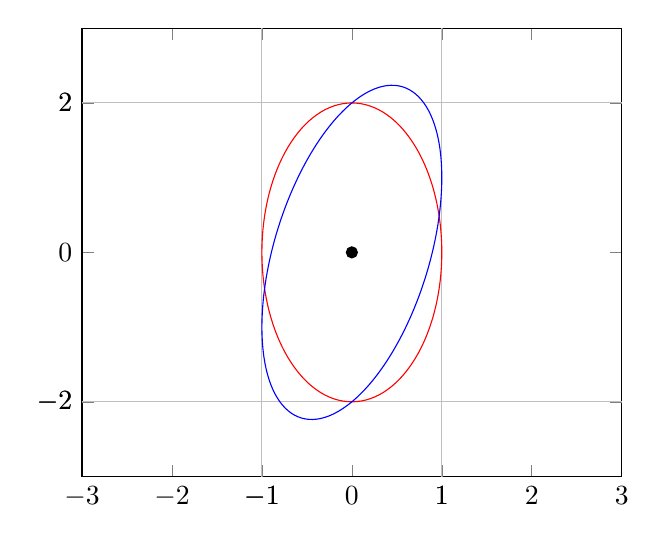
\begin{tikzpicture}
        \begin{axis}[
            xmin=-3,   xmax=3,
            ymin=-3,   ymax=3,
            extra x ticks={-1,1},
            extra y ticks={-2,2},
            extra tick style={grid=major},
        ]
            \draw[red] \pgfextra{
              \pgfpathellipse{\pgfplotspointaxisxy{0}{0}}
                {\pgfplotspointaxisdirectionxy{1}{0}}
                {\pgfplotspointaxisdirectionxy{0}{2}}
              % see also the documentation of
              % 'axis direction cs' which
              % allows a simpler way to draw this ellipse
            };
            \draw[blue] \pgfextra{
              \pgfpathellipse{\pgfplotspointaxisxy{0}{0}}
                {\pgfplotspointaxisdirectionxy{1}{1}}
                {\pgfplotspointaxisdirectionxy{0}{2}}
            };
            \addplot [only marks,mark=*] coordinates { (0,0) };
        \end{axis}
        \end{tikzpicture}
    \caption{My first autogenerated plot.}
  \end{center}
\end{figure}

\end{document}
\end{lstlisting}

\subsubsection{Kotlin minimal – Kotlin with pdflatex as a dependency}\label{subsubsec:kotlin_minimal}
This prototype uses Kotlin to satisfy platform-independence and invokes the pdflatex binary which is included in the TexLive distribution.
The project team chose to evaluate this technology because it satisfies the base requirements according to the project description and because
the project team is familiar with Kotlin.
Another advantage of this technology is that the distribution of the necessary LaTeX installation and packages is relegated to the user.
This greatly reduces distribution complexity.\newline
An obvious disadvantage of this approach is that the user needs to install TeXLive (and the pgfplots package) on their system, which might be difficult for non-technical users.

\paragraph{Licensing}\mbox{}\newline
This prototype is dependent on both TeXLive and pgfplots.
TeXLive uses a libre license that allows for the free redistribution with or without modifications~\cite{texlive_license} in accordance with the Free Software Foundation's free software definition~\cite{fsf_free_software}.
The pgfplots package uses the GPLv3 license~\cite{pgfplots}.

\paragraph{Evaluation}\mbox{}\newline
\begin{table}[H]
    \centering
    \begin{tabular}{l c c}
        \toprule
        \textbf{Criterion} & \textbf{Evaluation (1{-}5)} & \textbf{Weighted value} \\
        \midrule
        Know-how           & 4                           & 8                       \\
        \midrule
        Complexity         & 5                           & 20                      \\
        \midrule
        Usability          & 1                           & 6                       \\
        \midrule
        Distribution       & 5                           & 40                      \\
        \midrule
        \textbf{Total}     & n.a.                        & \textbf{74}             \\
        \bottomrule
    \end{tabular}
    \caption{Evaluation of Kotlin with pdflatex as a dependency}\label{table:kotlin_minimal_evaluation}
\end{table}

\subsubsection{Kotlin bundled – Kotlin bundled with pdflatex}\label{sec:kotlin_bundled}
Similarly to the prototype in~\fullref{subsubsec:kotlin_minimal}, this prototype uses Kotlin and invokes the pdflatex binary.
The major difference is that the pdflatex binary is provided alongside
the software.
The advantage of this approach is that the user does not have to install TexLive or any dependencies, greatly improving usability.
However, this comes with the disadvantage that the complexity of the distribution is much higher.
This approach also limits the advantages of using a platform-independent programming language because for every platform there has to be a release
which packages the appropriate binary.

\paragraph{Licensing}\mbox{}\newline
The licensing is equivalent to the licenses of the prototype in~\fullref{subsubsec:kotlin_minimal}.

\paragraph{Evaluation}\mbox{}\newline
\begin{table}[H]
    \centering
    \begin{tabular}{l c c}
        \toprule
        \textbf{Criterion} & \textbf{Evaluation (1{-}5)} & \textbf{Weighted value} \\
        \midrule
        Know-how           & 3                           & 6                       \\
        \midrule
        Complexity         & 3                           & 12                      \\
        \midrule
        Usability          & 5                           & 30                      \\
        \midrule
        Distribution       & 1                           & 8                       \\
        \midrule
        \textbf{Total}     & n.a.                        & \textbf{56}             \\
        \bottomrule
    \end{tabular}
    \caption{Evaluation of Kotlin bundled with pdflatex}\label{table:kotlin_bundled_evaluation}
\end{table}

\subsubsection{Web with SwiftLaTeX}
During the projects initial discussions, which had brainstorm like character, we wondered if we could render latex files directly in the browser, which would have the following benefits:
\begin{itemize}
    \item Providing the functionality as a web application would be probably the easiest and most accessible way for an end user to use the tool.
    \item Introducing the additional constraint of running the application only on the client side, would also avoid any infrastructure service and maintenance cost.
\end{itemize}
After a quick search we found the following open source JavaScript/WebWebassembly project: \href{https://www.swiftlatex.com/}{SwiftLaTeX: WYSIWYG LaTeX Editor for Browsers}
According to their website, the JavaScript/WebWebassembly library has the following characteristics~\cite{swiftlatex_website}:
\begin{itemize}
    \item 100\% Browser – PdfTeX and XeTeX written in WebAssembly and run in browsers.
    \item Compatibility – Produce exact same output you would get from TexLive or MikTeX\@.
    \item Library Support – Simply include a script tag and use PdfTeX or XeTeX in your own webpage.
    \item WYSIWYG – Support WYSIWYG editing on LaTeX documents using XeTeX engine.
    \item Speed – Run merely 2X slower than native binaries.
    \item Open Source – Completely Open Source. You can find the code on \href{https://github.com/SwiftLaTeX/SwiftLaTeX/}{GitHub}.
\end{itemize}
If the statements on the SwiftLaTeX website hold true, it would neatly full-fill our requirements for building a client side only web application.

\paragraph{Verifying basic functionality}\mbox{}\newline
To make a first feasibility test we can insert our reference LaTeX pgfplots template~\autoref{lst:reference_latex_pgfplots_template} into the \href{https://www.SwiftLaTeX.com/\#demo}{SwiftLaTeX Demo tool}.
Even though it took more than one and a half minute to process, we were very surprised that this just worked, see figure~\autoref{fig:SwiftLaTeX_demo_rendering_latex_pgfplots_template}:
\begin{figure}[H]
    \centering
    \includegraphics[width=0.5\textwidth]{SwiftLaTeX_demo_pgfplots}
    \caption{Screenshot of the SwiftLaTeX Demo tool rendering the reference LaTeX pgfplots template}\label{fig:SwiftLaTeX_demo_rendering_latex_pgfplots_template}
\end{figure}

\paragraph{Investigating dependencies are loaded}\mbox{}\newline
After investigating what actually happens on the page with the browsers developer tools network tab, we saw that SwiftLaTeX will load all dependencies asynchronously via https://texlive2.SwiftLaTeX.com/.
This process and how self-host those files, is documented in the README.md of the SwiftLaTeX GitHub library~\cite{SwiftLaTeX_github_repository}.
As we will be able to specify which LaTeX dependencies our application will use, it would be interesting to download and serve only the files we actually need.
We also saw that the dependencies are loaded sequentially, which we would like to optimize to reduce the pdf generation time.

\paragraph{Local development setup}\mbox{}\newline
To make the same example working on a local machine, we can download the latest release from the GitHub repository: \href{https://github.com/SwiftLaTeX/SwiftLaTeX/releases/tag/v20022022}{Releases 20/02/2022}.
The release contains the website visible at \href{https://www.SwiftLaTeX.com/}{SwiftLaTeX.com} including the compiled WebAssembly files.
As expected, opening the index.html file from the unzipped release folder in a browser will look like the website \href{https://www.SwiftLaTeX.com/}{SwiftLaTeX.com}.
Validating the basic functionality with our reference LaTeX pgfplots template~\autoref{lst:reference_latex_pgfplots_template} did not work, as we get the following error message in the JavaScript console:
\begin{lstlisting}[caption={SwiftLaTeX local development setup: JavaScript error message},label={lst:SwiftLaTeX_local_setup_js_error}]
PdfTeXEngine.js:89 Uncaught (in promise) SecurityError: Failed to construct 'Worker': Script at 'file:///home/lukas/Downloads/20-02-2022/SwiftLaTeXpdftex.js' cannot be accessed from origin 'null'.
...
\end{lstlisting}

According to the following \href{https://stackoverflow.com/questions/21408510/chrome-cant-load-web-worker}{stackoverflow question}, Google Chrome does not load web workers when running scripts from local files.
The web worker is required to run WebAssembly, which does all the actual LaTeX to PDF transformation in this prototype.
The easiest solution for this issue is to run a webserver, luckily this is trivial with Python.
We just have to run the following command in the directory of the unpacked SwiftLaTeX release folder:
\begin{lstlisting}[caption={Start a webserver on http://localhost:8000/ with Python},language=bash,label={lst:lstlisting}]
python -m http.server
\end{lstlisting}
Validating the basic functionality with our reference LaTeX pgfplots template~\autoref{lst:reference_latex_pgfplots_template} on http://localhost:8000/ works now as expected.

\paragraph{Distribution option 1: Python webserver}\mbox{}\newline
This would be the easiest solution, as it is analog to the local development setup described in the previous paragraph.
But installing Python, downloading the git repository or downloading a release and running the Python web server in the correct directory, requires at least a lot of technical affinity.

\paragraph{Distribution option 2: PyInstaller}\mbox{}\newline
To enhance the end users experience we could build an executable from a Python file with PyInstaller which supports builds for Windows, macOS and Linux.
Even though this solution worked in a quick proof of concept on a linux system, the user would need to find the public GitLab repository and download a release, which contains the latest executables.
Further the user might have security concerns, as downloading an executable from an unknown or untrusted source is really dangerous.

\paragraph{Distribution option 3: GitHub Pages}\mbox{}\newline
After thinking about it, we figured out that we could deploy the tool as a static HTML page to GitHub pages, this would resolve the need of downloading any source code or executable program.
In our opinion this would result in the best user experience, as the user only needs a web browser to access and use the tool.
As this solution was worth exploring, we deployed the prototype with GitHub pages: https://vonal3.github.io/

\paragraph{Licensing}
\begin{itemize}
    \item SwiftLaTeX:\ \href{https://github.com/SwiftLaTeX/SwiftLaTeX/blob/master/LICENSE}{SwiftLaTeX License}, \href{https://www.gnu.org/licenses/agpl-3.0.en.html}{GNU AFFERO GENERAL PUBLIC LICENSE}
    \item LaTeX:\ \href{https://www.latex-project.org/lppl.txt}{The LaTeX project public license}
    \item TeXLive:\ \href{https://www.tug.org/texlive/copying.html}{TeX Live licensing, copying, and redistribution}, \href{https://www.tug.org/texlive/LICENSE.TL}{COPYING CONDITIONS FOR TeX Live}
    \item pgfplots:\ \href{https://ctan.org/pkg/pgfplots}{https://ctan.org/pkg/pgfplots}, \href{https://www.gnu.org/licenses/gpl-3.0.en.html}{GNU General Public License, version 3 or newer}
\end{itemize}

\paragraph{Evaluation}\mbox{}\newline
\begin{table}[H]
    \centering
    \begin{tabular}{l c c}
        \toprule
        \textbf{Criterion} & \textbf{Evaluation (1{-}5)} & \textbf{Weighted value} \\
        \midrule
        Know-how           & 3                           & 6                       \\
        \midrule
        Complexity         & 3                           & 12                      \\
        \midrule
        Usability          & 4                           & 24                      \\
        \midrule
        Distribution       & 5                           & 40                      \\
        \midrule
        \textbf{Total}     & n.a.                        & \textbf{82}             \\
        \bottomrule
    \end{tabular}
    \caption{Evaluation of SwiftLaTeX JavaScript/WebAssembly library}\label{table:SwiftLaTeX_evaluation}
\end{table}

\subsubsection{Chosen Solution}
Using the evaluations given to the selected technologies, the following demonstrates the combined results:
\begin{table}[H]
    \centering
    \begin{tabular}{l c c}
        \toprule
        \textbf{Technology} & \textbf{Total score} \\
        \midrule
        Kotlin minimal      & 74                   \\
        \midrule
        Kotlin bundled      & 56                   \\
        \midrule
        Web SwiftLaTeX      & 82                   \\
        \bottomrule
    \end{tabular}
    \caption{Technology stack evaluation}\label{table:technology_evaluation}
\end{table}
In accordance with the table above, the project team decided to use \textbf{Web SwiftLaTeX} with the distribution option 3 \textbf{GitHub Pages}.

\subsection{License}\label{subsec:evaluation-license}
After evaluating the different possible technologies, the following third party software will be used:
\begin{itemize}
    \item SwiftLaTeX: \href{https://github.com/SwiftLaTeX/SwiftLaTeX/blob/master/LICENSE}{SwiftLaTeX License}, \href{https://www.gnu.org/licenses/agpl-3.0.en.html}{GNU AFFERO GENERAL PUBLIC LICENSE}
    \item LaTeX: \href{https://www.latex-project.org/lppl.txt}{The LaTeX project public license} (GPL Compatible)
    \item TeXLive: \href{https://www.tug.org/texlive/copying.html}{TeX Live licensing, copying, and redistribution}, \href{https://www.tug.org/texlive/LICENSE.TL}{COPYING CONDITIONS FOR TeX Live} (GPL Compatible)
    \item pgfplots: \href{https://ctan.org/pkg/pgfplots}{https://ctan.org/pkg/pgfplots}, \href{https://www.gnu.org/licenses/gpl-3.0.en.html}{GNU General Public License, version 3 or newer}
    \item Bootstrap: \href{https://github.com/twbs/bootstrap/blob/main/LICENSE}{Bootstrap License}, \href{https://en.wikipedia.org/wiki/MIT_License}{MIT License} (GPL Compatible)
\end{itemize}
To be conform with the used software, we will also publish our code under the \href{https://www.gnu.org/licenses/gpl-3.0.en.html}{GPL-3.0 licence (FLOSS)}.

    \section{Implementation}
Lorem ipsum

\subsection{Architecture}
Lorem ipsum

\subsection{Processes}
Lorem ipsum


    \section{Deployment and Integration}\label{sec:deployment-and-integration}
We decided to use GitHub Pages via an \href{https://github.com/decibel-threshold-event-displayer}{organization} for distribution because it provides an easy way to access the
application for end users and simplifies the maintenance for developers. The application is then available as a \href{https://decibel-threshold-event-displayer.github.io/}{Github Page}.
The following list and the graphic~\autoref{fig:deployment_flow} elaborates on the deployment workflow.

\begin{enumerate}
    \item A dev pushes or merges code to the main branch
    \item GitLab automatically mirrors the repository to GitHub
    \item GitHub deploys automatically to GitHub Pages
    \item {The Application is available under: \\
          \href{https://decibel-threshold-event-displayer.github.io/}{https://decibel-threshold-event-displayer.github.io/}}
\end{enumerate}

\begin{figure}[H]
    \centering
    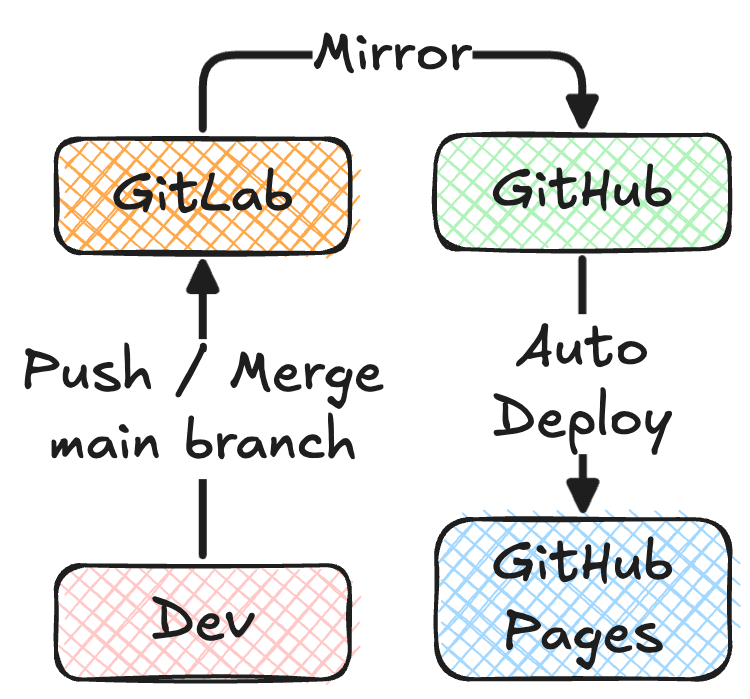
\includegraphics[width=0.5\textwidth]{../assets/deployment_and_distribution.png}
    \caption{Deployment Flow}\label{fig:deployment_flow}
\end{figure}

\subsection{Installation Manual \& Script}\label{subsec:installation-manuel-and-script}
We are using a Makefile to automate the development setup, build and deploy the application to GitHub Pages.

\subsubsection{Development setup}\label{subsubsec:deployment-setup}
A local webserver is needed work on the application as some Browsers will not execute web workers on locally served files~\cite{stackoverflow_chrome_cant_load_web_worker}.
By default, the project uses the built-in webserver of Python 3.
Python 3 can be installed with the systems package manager or by downloading it from the \href{https://www.python.org/downloads/}{official website}.
Afterward the following command can be used to run the local webserver on \href{http://0.0.0.0:8000/}{0.0.0.0:8000/\#/}:

\begin{lstlisting}[caption={Makefile: Start local webserver},label={lst:makefile_start_local_webserver},language=Bash]
$ make dev
\end{lstlisting}

\subsubsection{Distribution}
The project and the repository is managed via the GitLab of BFH,
but we want to use GitHub pages to deploy and distribute our application,
the project team decided that we mirror the GitLab repository to GitHub:
\begin{itemize}
    \item \href{https://gitlab.ti.bfh.ch/decibel-threshold-event-displayer/decibel-threshold-event-displayer}{GitLab Repository}
    \item \href{https://github.com/decibel-threshold-event-displayer/decibel-threshold-event-displayer.github.io}{GitHub Repository}
\end{itemize}

\paragraph{Mirror setup:}
\begin{enumerate}
    \item Log into \href{https://gitlab.ti.bfh.ch}{gitlab.ti.bfh.ch}
    \item Navigate to the repository: \href{https://gitlab.ti.bfh.ch/decibel-threshold-event-displayer/decibel-threshold-event-displayer/}{GitLab Repository}
    \item Go to the repositories settings page: \href{https://gitlab.ti.bfh.ch/decibel-threshold-event-displayer/decibel-threshold-event-displayer/-/settings/repository}{Settings > Repository}
    \item Open the Tab ``Mirroring repositories``
    \item Click the button ``Add new``
    \item Fill the form as follows:
          \begin{itemize}
              \item Git repository URL: ssh://git@github.com/decibel-threshold-event-displayer/decibel-threshold-event-displayer.github.io.git
              \item Mirror direction: Pull
              \item Authentication method: SSH public key
              \item Username: github
              \item Mirror user: autofilled
              \item Overwrite diverged branches: Select
              \item Mirror branches > Mirror specific branches: main
          \end{itemize}
    \item Click the button ``Mirror repository``
    \item The first try will fail, as we have to add the public key generated by GitLab to the GitHub repository
    \item On the newly created entry, click the clipboard button ``Copy SSH public key`` (the public key is now in your clipboard)
    \item Keep the current GitLab tab open
    \item Log into \href{https://github.com/}{github.io} in a new tab
    \item Navigate to the repository: \href{https://github.com/decibel-threshold-event-displayer/decibel-threshold-event-displayer.github.io/}{GitHub Repository}
    \item Go to the repositories deploy keys page: \href{https://github.com/decibel-threshold-event-displayer/decibel-threshold-event-displayer.github.io/settings/keys}{Settings > Deploy Keys}
    \item Click the button ``Add deploy key``
    \item Fill the form as follows:
          \begin{itemize}
              \item Title: github
              \item Key: Copy the SSH public key from the clipboard
              \item Allow write access: yes
          \end{itemize}
    \item Click the button ``Add Key``
    \item Go back to the gitlab tab
    \item Click the reload button ``Update now``
    \item Wait until the process is finished
\end{enumerate}

\subsubsection{Build}
As we have only plain JavaScript files, we don't have a build step.

\subsubsection{Deploy}
As described above, we created a Mirror of this repository on GitHub.
Based on the following documentation, we configured GitHub to automatically deploy to GitHub Pages:
\href{https://docs.github.com/en/pages/getting-started-with-github-pages/creating-a-github-pages-site}{Creating a GitHub Pages site}

Further we had to add a configuration file under ``.github/workflows/static.yml`` and change value of \texttt{path: './'} to \texttt{path: './app'}.
The initial file was generated by the following setup page:
\href{https://github.com/decibel-threshold-event-displayer/decibel-threshold-event-displayer.github.io/new/main?filename=.github%2Fworkflows%2Fstatic.yml&pages_workflow_template=pages%2Fstatic}{Repository > Settings > GitHub Pages > Static HTML > Configure}

\subsection{User Manual}\label{subsec:user-manuel}
The project team decided to not create an additional document for the user manual,
because all the necessary information for using the application are provided by following list of best practices:
\begin{itemize}
    \item Following common UI patterns
    \item Well-known form components
    \item Tooltips where needed
    \item Human-readable error messages
    \item About page with detailed technical information
\end{itemize}


    \part{Scrum}
    \section{Scrum Roles}\label{sec:scrum_roles}
The project team has, in coordination with the tutor, determined that the association Lärmliga (\url{https://laermliga.ch/}) will not be directly involved
in the project.
Instead, the tutor Dr.\ Simon Kramer, will take on the role of the stakeholder and render the decisions to be made by the customer. \\
The other scrum roles were determined internally by the project team.
At first, the decision was made for Dr.\ Simon Kramer to also be the Product Owner.
However, the project team realized it would be impractical to include Dr.\ Simon Kramer in every product decision and especially in the prioritization of the backlog.
The project team felt that, due to their relative inexperience, it would be best to have the Product Owner in the team, so decisions could be made quickly and validated
with the stakeholders afterward, if necessary.
\begin{table}[H]
    \centering
    \begin{tabular}{l l}
        \toprule
        \textbf{Name}     & \textbf{Role(s)}         \\
        \midrule
        Dr.\ Simon Kramer & Stakeholder, Tutor       \\
        \midrule
        Dominic Gernert   & Product Owner, Developer \\
        \midrule
        Lukas von Allmen  & Scrum Master, Developer  \\
        \midrule
        Darius Degel      & Developer                \\
        \bottomrule
    \end{tabular}
    \caption{Scrum Roles}\label{table:scrum_roles}
\end{table}
    \section{Sprint Goals}
The sprint goals are defined by the project team at the Sprint Planning right after the conclusion of the previous sprint.
They are formulated to be compliant with the S.M.A.R.T principles. The project team decides the sprint goals based on the backlog
priorisation and the issues assigned to the next sprint. The sprint goals are defined and reviewed in a Markdown file in the repository (\href{https://gitlab.ti.bfh.ch/decibel-threshold-event-displayer/decibel-threshold-event-displayer/-/blob/main/doc/scrum/sprints.md}{Gitlab}).
\subsection{Sprint 1}
For the first sprint, the project team decided to focus on research and prototyping. This can be understood as a feasibility study.
Due to the team's relative inexperience with LaTeX and due to the project scope, they felt that having a working prototype had to be
made before design decision could realistically be made. \\
\begin{table}[H]
    \centering
    \begin{tabularx}{\textwidth}{X c}
        \toprule
        \textbf{Goal}                                                                                    & \textbf{Reached} \\
        \midrule
        Prototypes with two different technologies are implemented and their pros and cons are evaluated & Yes              \\
        \midrule
        Tech stack for the project has been chosen                                                       & Yes              \\
        \midrule
        Licence is defined                                                                               & No               \\
        \midrule
        Git repository and documentation skeleton are created                                            & No               \\
        \bottomrule
    \end{tabularx}
    \caption{Sprint Goals of Sprint 1}\label{table:sprint_goals1}
\end{table}
In Sprint 1, the project team managed to complete the first two goals (prototyping and tech stack evaluation). However, they were unable to
evaluate the licencing because the decision, which tech stack should be used was made only at the end of the sprint. The project team als underestimated
the issue weights, leading to unreached goals.
\subsection{Sprint 2}
Sprint 2 has not ended, as of the completion date of this document. Nonetheless, two of the seven defined sprint goals have been reached at this point.
Although the project team defined more goals for the second sprint than the first, it is important to note that the total weight of tasks assigned to this
sprint is equal to the first sprint and estimates are more conservative.
\begin{table}[H]
    \centering
    \begin{tabularx}{\textwidth}{X c}
        \toprule
        \textbf{Goal}                                         & \textbf{Reached} \\
        \midrule
        Intermediate presentation is prepared and presented   & n.a.             \\
        \midrule
        Requirements are specified                            & n.a.             \\
        \midrule
        UX-Prototype is defined                               & n.a.             \\
        \midrule
        System delimitation is specified                      & n.a.             \\
        \midrule
        Decibel values can be calculated                      & n.a.             \\
        \midrule
        Licence is defined                                    & Yes              \\
        \midrule
        Git repository and documentation skeleton are created & Yes              \\
        \bottomrule
    \end{tabularx}
    \caption{Sprint Goals of Sprint 2}\label{table:sprint_goals2}
\end{table}
    \section{Requirements}
\subsection{Epics}
Epics were defined at the very beginning of the project and are largely product focussed.
Epics are defined in the Epics section of the Planning tab in Gitlab (\href{https://gitlab.ti.bfh.ch/groups/decibel-threshold-event-displayer/-/epics}{Gitlab}). Epics are subject to change
but for the sake of completeness, they are included in this document anyway (see \autoref{fig:epics}).
\begin{figure}[H]
    \centering
    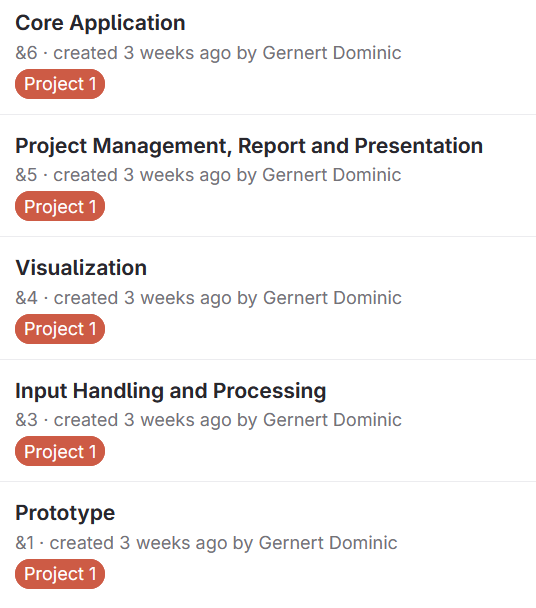
\includegraphics[width=0.5\textwidth]{epics_interim_presentation.png}
    \caption{Epics}\label{fig:epics}
\end{figure}
\subsection{User Stories}
User Stories are created as Issues in Gitlab. They are associated with an Epic and are prioritised. Issues contain a \textit{Definition of Ready} (\ref{subsubsec:dor}), Acceptance Criteria, as well as a \textit{Definition of Done} (\ref{subsubsec:dod}).
When an issue is selected for a sprint, sub-tasks are created, estimated and assigned. The issue itself is assigned to the person with the most assigned sub-tasks. The full list of issues is available in \href{https://gitlab.ti.bfh.ch/groups/decibel-threshold-event-displayer/-/issues}{Gitlab's issue list} or the \href{https://gitlab.ti.bfh.ch/decibel-threshold-event-displayer/decibel-threshold-event-displayer/-/boards/2832}{Development Board}.

\subsubsection{Definition of Ready}\label{subsubsec:dor}
The \textit{Definition of Ready} is defined as a checklist on every User Story. In every Sprint Planning the issues selected for
the next sprint are validated by crossing off the checklist. All necessary adjustments are made together by the project team before the issue is
estimated and planned. The \textit{Definition of Ready} is part of the issue template in the repository
(see \href{https://gitlab.ti.bfh.ch/decibel-threshold-event-displayer/decibel-threshold-event-displayer/-/blob/main/.gitlab/issue_templates/User\%20Story.md}{Gitlab}). \\ \\
\textit{Definition of Ready}:
\begin{itemize}
    \item Requirements and Acceptance Criteria Defined
    \item Acceptance Criteria must be testable
    \item Understood by the Team
    \item Sized and Estimated
    \item Prioritized in the Backlog
    \item No Major Impediments
\end{itemize}
\subsubsection{Definition of Done}\label{subsubsec:dod}
Similarly to the \textit{Definition of Ready} (\ref{subsubsec:dor}),  the \textit{Definition of Done} is a static checklist that is part of
the issue template. The tasks are checked off by the reviewer, which is the Product Owner unless specified otherwise. \\ \\
\textit{Definition of Done}:
\begin{itemize}
    \item Acceptance Criteria Met
    \item Tested and no Critical Bugs
    \item Documentation Updated
    \item Reviewed and Approved
\end{itemize}
\subsection{Product Backlog}\label{subsec:product_backlog}
Issues are prioritised first and foremost by the Product Owner. This priorisation is implemented as tags in Gitlab and is can be viewed
on the \href{https://gitlab.ti.bfh.ch/decibel-threshold-event-displayer/decibel-threshold-event-displayer/-/boards/2832}{Development Board} (see\ \autoref{fig:product_backlog})
\begin{figure}[H]
    \centering
    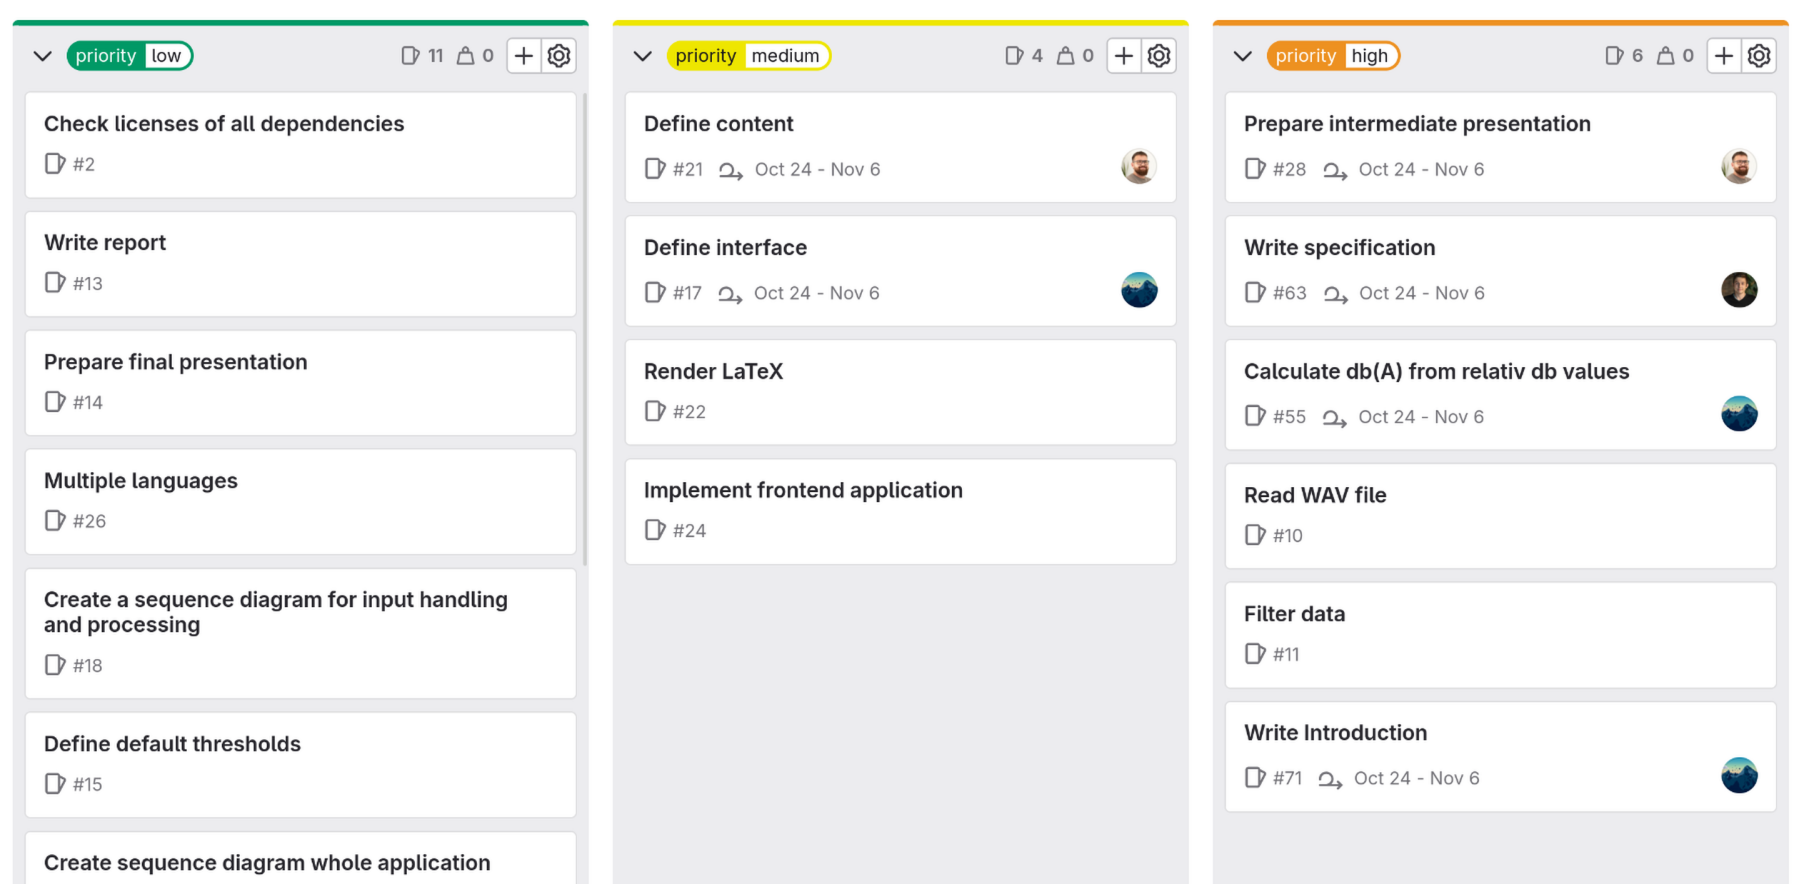
\includegraphics[width=\textwidth]{product_backlog.png}
    \caption{Product Backlog}\label{fig:product_backlog}
\end{figure}
\subsection{Sprint Backlog}
The Sprint Backlog of the currently running sprint is displayed as a column on the \href{https://gitlab.ti.bfh.ch/decibel-threshold-event-displayer/decibel-threshold-event-displayer/-/boards/2832}{Development Board}. In combination with the priorisation (see\ \ref{subsec:product_backlog}),
this makes for a convenient way for the project team to select issues for the next sprint based on priority (see\ \autoref{fig:sprint_backlog}).
\begin{figure}[H]
    \centering
    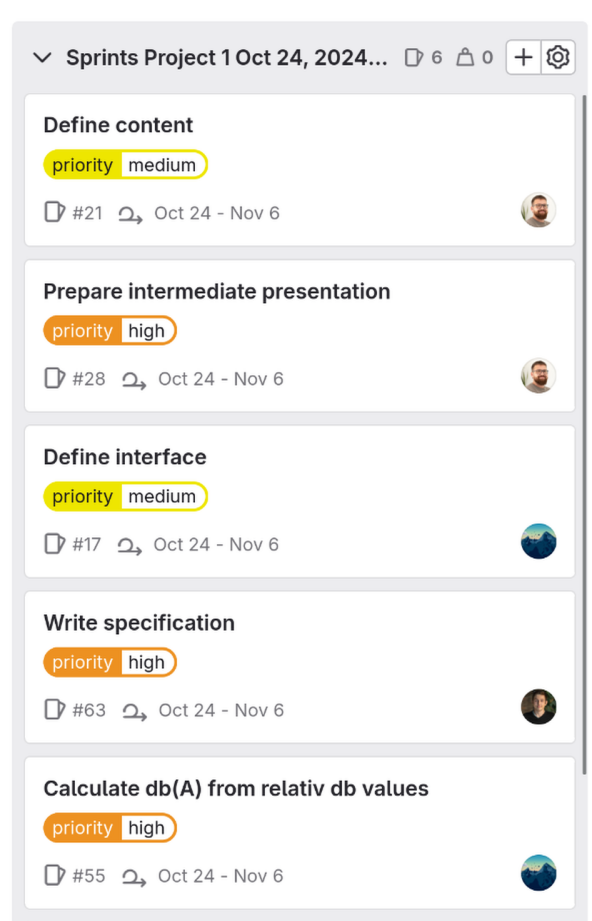
\includegraphics[width=0.5\textwidth]{sprint_backlog_sprint2.png}
    \caption{Sprint Backlog}\label{fig:sprint_backlog}
\end{figure}
\subsection{Impediment Backlog}\label{subsec:impediment_board}
Impediments are also created as Issues in Gitlab. They are however, assigned the label \textit{Impediment} and are displayed on a separate Impediment Board (see\ \autoref{fig:impediment_board} and \href{https://gitlab.ti.bfh.ch/decibel-threshold-event-displayer/decibel-threshold-event-displayer/-/boards/2834?label_name[]=impediment}{Gitlab}).
Impediments are created either ad hoc or during the Daily Standup meeting. There is a template for Impediments analogous to the Issue template (see \href{https://gitlab.ti.bfh.ch/decibel-threshold-event-displayer/decibel-threshold-event-displayer/-/blob/main/.gitlab/issue_templates/Impediment.md}{Gitlab}).
\begin{figure}[H]
    \centering
    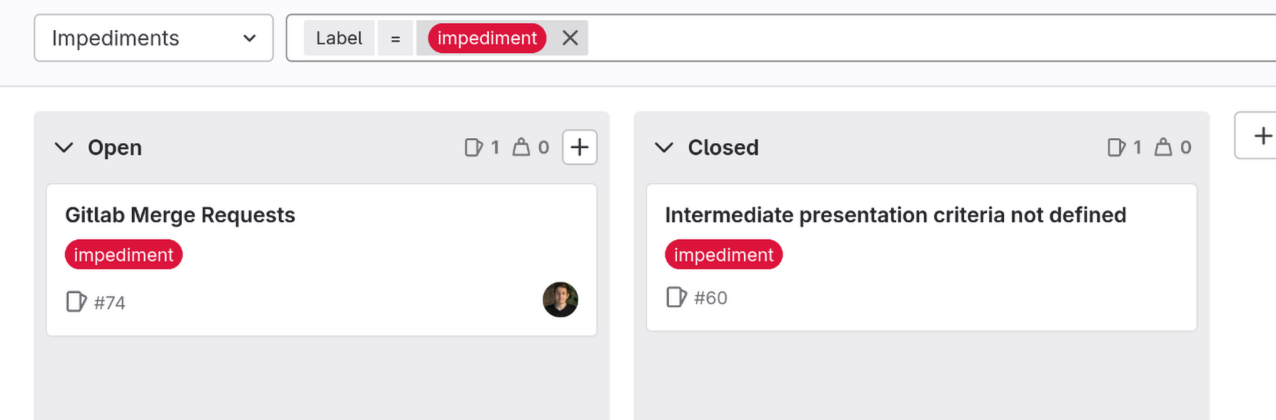
\includegraphics[width=\textwidth]{impediment_board.png}
    \caption{Impediment Board}\label{fig:impediment_board}
\end{figure}
    \section{Scrum Adaptations}\label{sec:scrum-adaptations}
\subsection{Product Owner}\label{subsec:product-owner}
As described in \autoref{sec:scrum_roles}, the Product Owner role has gone from our tutor, Dr.\ Simon Kramer, to Dominic Gernert.
Although not specifically mentioned in the Scrum Guide\cite{scrum_guide}, in the experience
of the project team and an article on applied frameworks\cite{applied_frameworks_po}, the Product Owner is usually someone with a business background and not a developer.
This makes sense, because they need to be able to make decisions about the product that only a business expert could make.
Since this is not the real world but a school project, the project team had to reduce the coordination effort.
Thus, the team decided to make Dominic Gernert the Product Owner.
Since he is not a business expert for our project, decisions are still made as a collective.
If however, there is a disagreement on a decision, the Product Owner's suggestion is followed.
For bigger decisions,the Stakeholder Dr.\ Simon Kramer is involved.
\subsection{Daily Scrum}\label{subsec:daily-scrum}
As suggested by Mr.\ Frank Helbling in the Scrum presentation\cite{helbling_scrum3}, the project team has decided to confine their Daily Scrum to 15 minutes.
They are scheduled weekly on Wednesday at 18:15.
The Scrum meetings that took place until the completion date of this document took about 30 minutes, however.
The likely reason for this is that the project team meets only weekly,
but each person actually works on the project at multiple days of the week.
This leads to more information, questions, and impediments being generated and having to be discussed during the Daily Scrum.
The project team is still trying to keep their Daily Scrum short (less than 20min.) in the future.
\subsection{Release Plan}\label{subsec:release-plan}
The project team has decided against implementing a Release Plan.
Mainly because it was never explicitly demanded by the tutor, Dr.\ Simon Kramer.
The other reason for forgoing the Release Plan is that
there is no real customer awaiting product updates and Dr.\ Kramer is capable of running the application himself should he want to do so.
Product demonstrations by the team are not on a fixed scheduled and
are done if necessary or requested by the stakeholder.
\subsection{Retro}\label{subsec:retro}
Instead of following the Keep-Try-Drop model for the Sprint Retrospective, the project team decided to focus on successes, problems, and improvements.
A reason for that is the focus on the individual by the team due to the low number of members.
This focus on successes and problems provides a way for each team member to explain their frustrations and discuss possible improvements.
This adaptation is comparatively small and mostly one of wording.
The project team feared however, that using the Keep-Try-Drop model, they would have to justify using certain tools when running into minor problems.
Instead, the team hopes to focus more on the product than the tool chains.
    \section{Project Setup Review}\label{sec:project-setup-review}
% Erfassung der Ausgangssituation, Themen-Analyse, Stakeholder(-Management), Organisation, Installationen
% Identifying the initial situation, topic analysis, stakeholder (management), organisation, installations

\subsection{Identifying the initial situation}\label{subsec:identifying-the-initial-situation}
For identifying the initial situation we analysed~\fullref{subsec:project-description} and used multiple online resources
such as the websites of \href{https://laermliga.ch/}{Lärmliga Schweiz} and \href{https://www.bafu.admin.ch/bafu/en/home/topics/noise/in-brief.html}{Federal Office for the Environment FOEN}.
Based on those information we were able to derive some of the requirements and specifications for our application,
which now provides a convenient way for affected people to document noise pollution.

\subsection{Topic analysis}\label{subsec:topic-analysis}
To solve the issue at hand, one needs knowledge about how audio recoding and measurement works.
We invested the time needed to analyse the topic and gather the know-how needed to process and analyse audio files.
A short summary of the problematic can be found under~\fullref{subsec:problems-with-audio-files}.
This analysis provided the technical basis for achieving the product goal.

\subsection{Stakeholder / Stakeholder Management}\label{subsec:stakeholder-management}
Initially we identified a list of possible stakeholders:

\begin{itemize}
    \item Tutor: Dr. Simon Kramer
    \item People affected by noise pollution
    \item Noise producers (Construction Sites, Night Clubs, Highways)
    \item Lärmliga Schweiz
    \item Federal Office for the Environment FOEN
\end{itemize}

For the context of this module we decided to only consider our tutor as the sole stakeholder,
because otherwise the stakeholder management would cost much more time without much benefit.
This way the stakeholder management turned out to be straight forward, as Dr. Kramer provided his expectations and the
scope of the project beforehand, only impediments and key decisions had to be discussed together.

\subsection{Organisation}\label{subsec:organisation}
The project organisation and how the project team implemented scrum is documented under the following three chapters:

\begin{itemize}
    \item \fullref{sec:scrum_roles}: The distribution of the Scrum Roles has been proven practicable even though some of the project members didn't have any experience in their respective roles
    \item \fullref{sec:scrum-adaptations}: The project team was really happy about the way we adapted Scrum in this project as it was really product focused and did not introduce too much overhead
    \item \fullref{sec:requirements}: We found especially the definition of ready and the definition of done where really helpful, as it made sure the tickets had a minimum quality, are well understood and had a clear achieveable goal.
\end{itemize}

Further the project team mainly worked together remotely which reduced the unnecessary over head of commuting.



    \section{Review}\label{sec:review}
% Produktziel erreicht? Sprintziele? Abgrenzung? Lieferobjekte erstellt? Product Backlog / Sprint Backlogs?
% Product target achieved? Sprint targets? Delimitation? Deliverables created? Product backlog / sprint backlogs?

\subsection{Product goals}\label{subsec:product-goals-review}
The following list summarizes the~\ref{subsec:product-goals} Product goals:

\begin{enumerate}
    \item Analyze Audio File
    \item Summarize findings in a PDF
    \item Easy to use
\end{enumerate}

From our point off view, the first two Product goals are clearly achieved, as we built a working application
which can parse and analyze Audio Files and then summarizes the findings in a PDF document.
The third goal `Easy to use` is not as easy to measure, but we argue that this is achieved by considering the following
list of best practices:

\begin{enumerate}
    \item Cross platform: Achieved by building a public web application
    \item No login or other personal data required
    \item Clarity, consistency, responsiveness and familiar patterns: Achieved by using~\href{https://getbootstrap.com/2.0.2/}{Bootstrap, from Twitter}
    \item Help and documentation: Achieved with integrating tooltips where needed and show human-readable error messages
    \item Performance and fast load times: Achieved by realizing the application as a minimal SPA and preloading all necessary LaTeX resources in the background as the user is already filling out the form
\end{enumerate}

\subsection{Sprint goals}\label{subsec:sprint-goals-review}


\subsection{Product delimitation}\label{subsec:product-delimination-review}


\subsection{Deliverables}\label{subsec:deliverables-review}


\subsection{Product backlog / sprint backlogs}\label{subsec:backlog-review}


    \section{Retrospective}\label{sec:retrorespective}

\subsection{Retrospective I: Scrum roles and stakeholders}\label{subsec:retrospective-scrum-roles-and-stakeholder}
% Scrum Roles und Stakeholder: Erfahrungen und Fazite zu Scrum Roles (Product Owner, Scrum Master, Developer) und weiteren Stakeholder.
% Scrum roles and stakeholders: Experiences and conclusions on Scrum Roles (Product Owner, Scrum Master, Developer) and other stakeholders.

\begin{itemize}
    \item Product Owner: Dominic already has quite some experience with Scrum and thus made a perfect job from the beginning.
    \item Scrum Master: Even though Lukas held the role for the first time he could fulfill it after a bit of initial support from Dominic.
    \item Developers: Thanks to the clear definition of ready and definition of done, the developers always knew what to do in every task.
    \item Stakeholder: The project team enjoyed working with Dr. Kramer as the expectations were communicated beforehand and clearly.
\end{itemize}

\subsection{Retrospective II: Scrum Events and Artifacts}\label{subsec:retrospective-scrum-events-and-artifacts}
% Scrum Events und Artifacts: Erfahrungen und Fazite zu Scrum Events und Scrum Artifacts.
% Scrum Events and Artifacts: Experiences and conclusions on Scrum Events and Scrum Artifacts.

\begin{itemize}
    \item Product Backlog: The Product Owner did a perfect job with specifying and managing the product backlog. This helped the team to progress without any blockers.
    \item Sprint planning meeting: The planning was always really smooth, as it was clear which the logical next steps are.
    \item Sprint backlog: The Sprint backlogs were always a bit overambitious, as we almost never achieved all the sprint goals.
    \item Daily Scrum meetings: The 'Dailies' were actually held once a week, nevertheless they helped us to resolve issues on the current tasks and kept all team members in sync.
    \item Burndown Charts: As we did not work on the project every day, the burndown charts looked not like a gradual line downwards but instead showed a clear trend of the team doing work on weekends and within the time slot of the Proejct 1 module.
    \item Finished work: As we had a clear definition of done, the finished work was always documented in the projects report.
    \item Sprint Review: The project team really enjoyed the sprint reviews, as it made the progress visible.
    \item Sprint Retrospective: At the start of the project, we decided to use a minimal approach for the retrospective and the project team was really happy with this decision.
\end{itemize}

\subsection{Retrospective III: Tools/Instruments}\label{subsec:retrospective-tools-instruments}
% Tools/Instrumente: Erkenntnisse zu Tool-Einsatz (GitLab/GanttLab, Teams, etc.) und Controlling (Burndown Chart, etc.).
% Tools/Instruments: Findings on tool use (GitLab/GanttLab, teams, etc.) and controlling (burndown chart, etc.).

\begin{itemize}
    \item GitLab: The project team was not always happy with the workflows provided by GitLab, such as the issue boards and the differentiation between group and project.
    \item MS Teams: This tool is an amazing, unified communication channel for working together, but the Linux support could be better.
    \item \href{https://www.microsoft.com/en-us/microsoft-365/outlook/email-and-calendar-software-microsoft-outlook}{MS Outlook}: MS Outlook just works as expected.
    \item LaTeX: Even though we did not have a lot of experience with LaTeX, we decided to use it for all documentation and presentation purposes.
          The project team enjoyed working with LaTeX, but for non-academic contexts we would have chosen less complex tools such as MS Word and MS PowerPoint.
    \item \href{https://excalidraw.com/}{Excalidraw}: This easy to use online tool helped us to create a lot of the diagrams and UI-Prototypes.
    \item \href{https://www.drawio.com/}{draw.io}: Another easy to use online tool for creating diagrams where the results look a bit more old-school / professional.
    \item Controlling:
          \begin{itemize}
              \item Burndown Chart: The Burndown chart was a good visual indicator to see how the sprints progress is going, but as we often underestimated tasks it could be quite misleading for an external observer.
              \item Product Backlog: Thanks to the detailed initial product backlog we could always see where we stood in the project.
          \end{itemize}
\end{itemize}
    \section{Lessons learned}\label{sec:lessons-learned}
% Erkenntnisse zu Rahmenbedingungen, Zusammenarbeit (im Team, Fachbetreuer, PM-Coach, Kunde, Betreiber, etc.)
% Insights into framework conditions, cooperation (in the team, specialist advisor, PM coach, customer, operator, etc.)

\subsection{Insights into framework conditions}\label{subsec:insights-into-framework-conditions}
For the team members which already had quite some experience with Scrum,
there was still the learning curve of setting up everything from scratch.
The other member had quite some experience with alternative forms of agile software development and could learn a lot about the Scrum specific methods.
In our point of view, the most important Scrum ceremonies were the sprint review and planning
which we always held subsequently.
The sprint review resulted in some interesting demos, kept the whole team in sync, showed the current progress, and
already indicated what the next steps could be.
On the other hand there is no sprint without the sprint planning and after it, every team member knows what he has to do next.
In the context of project 1 the key takeaway for the project team is, that Scrum also works when nobody works full-time
on the project and all the work is done remotely.

\subsection{Cooperation}\label{subsec:cooperation}
\paragraph{Team:}
The key challenge for the project team in terms of cooperation was the limbo between working, other modules, and project 1.
This resulted in the reality that we only worked together in the modules official time block.
In the beginning a project member had issues being on time for meetings, but luckily he could resolve this issue.
Besides the minor challenges and issues, the team work was amazing, and we enjoyed working together.

\paragraph{Specialist advisor / Stakeholder:}
We consider the cooperation with Dr. Kramer as good, as he communicated his expectations clearly from the start.
If we had issues or questions we received an answer within reasonable time or could schedule a meeting with him in the
modules official time block.

\paragraph{Project Management Coach:}
The cooperation needed with the project management coach was minimal as all requirements were clearly documented in moodle.
When something was unclear we received an answer within reasonable time.

    \part{Conclusion}
    \begin{frame}
    \frametitle{Conclusion}
\end{frame}
    \section{Glossary}


    \section{Bibliography}
Lorem ipsum

    \section{Appendix}\label{sec:appendix}

\subsection{Project description}\label{subsec:project-description}

The \textbf{goal (what)} of this project is to deliver a FLOSS-licensed, platform-independent piece of
software (computer program), called the \textit{Decibel Threshold Event Displayer}, that

\begin{enumerate}
    \item takes as inputs a WAV-file and a list of sound level thresholds in decibels (e.g., legal day
          and nighttime noise maxima above which your health deteriorates);
    \item filters out all data points in the file that correspond to sound events below the lowest of
          the above thresholds; and
    \item displays the remaining data points (as a blue vertical comb plot) on a horizontal time
          axis (with the dates and times corresponding to the data points) as well as the
          thresholds (as horizontal red lines) in decibel, and statistically summarises the data set
          with the help of the LaTeX-package pgfplots.
\end{enumerate}

The \textbf{purpose (why)} of this project is to empower poor folks who suffer from insomnia due to
ambient noise (\url{https://laermliga.ch/}) by arming them with the (peaceful) means of proving
their noise hell (a smartphone app such as \url{https://apps.apple.com/ch/app/dezibel-x-pro-l\%C3\%A4rm-messger\%C3\%A4t/id1257651611}
together with your software) to the police and the courts of law. \\

The code should be minimal, modular, and self-explaining. \\

The project report should be concise (maximally informative, minimally long). It must contain
this project description as a quotation.

\subsection{Declaration of Authorship}\label{subsec:declaration-of-authorship}
The project team, namely Dominic Gernert, Lukas von Allmen, and Darius Degel, hereby declare that the report submitted is our own unaided work.
All direct or indirect sources used are acknowledged as references.
\end{document}
